\documentclass[12pt]{article}

\usepackage[utf8]{inputenc}
\usepackage[english]{babel}
\usepackage[margin=1in]{geometry}
\usepackage{graphicx}
\usepackage{pdfpages}
\usepackage{hyperref}
\usepackage{bookmark}

\begin{document}

\begin{titlepage}
  \centering
  \vspace*{2in}
  {\huge CO342 - Introduction to Graph Theory}\par
  {\Large (Notes Scans)}\par
  \vspace{0.3in}
  {\large University of Waterloo}\par
  {\large Nicholas Pun}\par
  {\large Fall 2017}\par 
\end{titlepage}
 
\tableofcontents
\clearpage

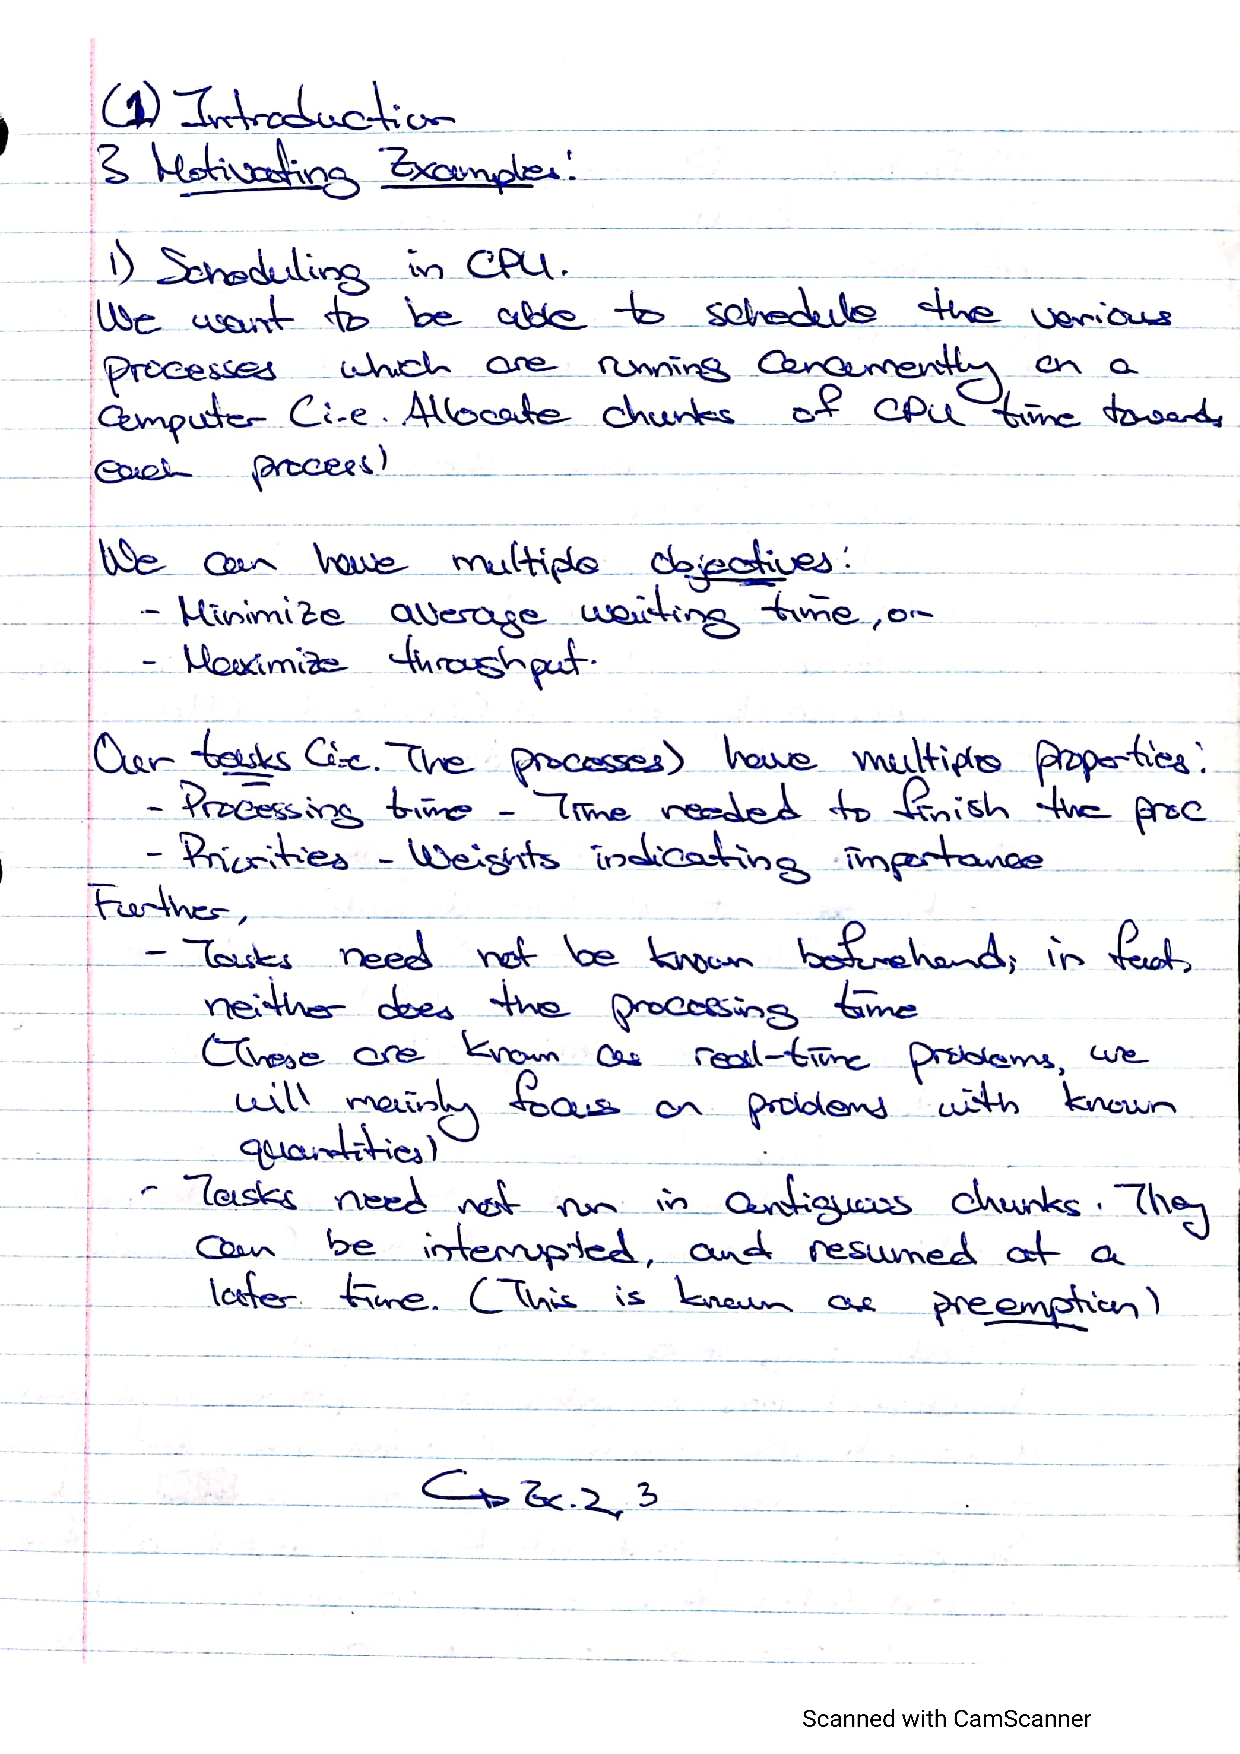
\includepdf[pages=1, pagecommand={\thispagestyle{plain}\section{Connectivity}}]{sections/sec1.pdf}
\includepdf[pages=2-, pagecommand=\thispagestyle{plain}]{sections/sec1.pdf}
\clearpage

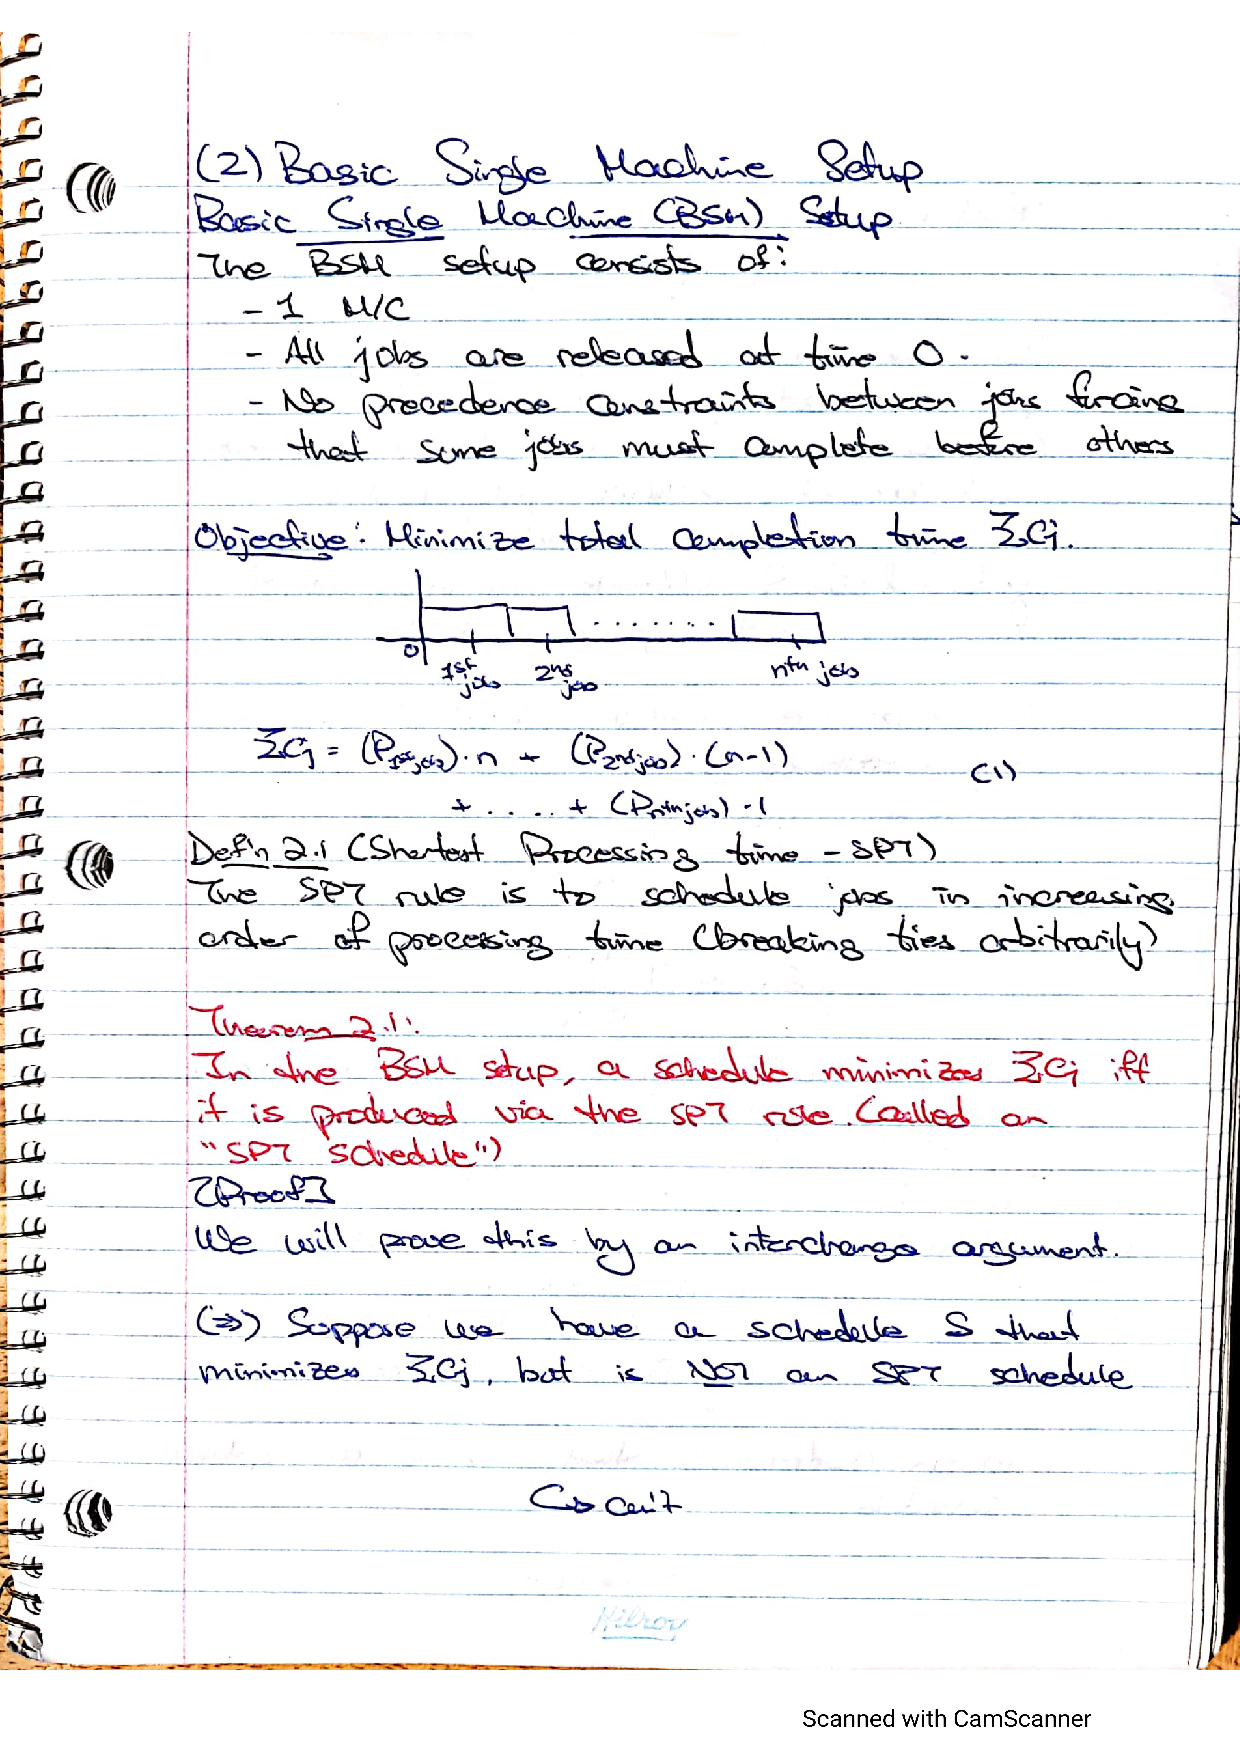
\includepdf[pages=1, pagecommand={\thispagestyle{plain}\section{Vector Spaces for Graphs}}]{sections/sec2.pdf}
\includepdf[pages=2-, pagecommand=\thispagestyle{plain}]{sections/sec2.pdf}
\clearpage

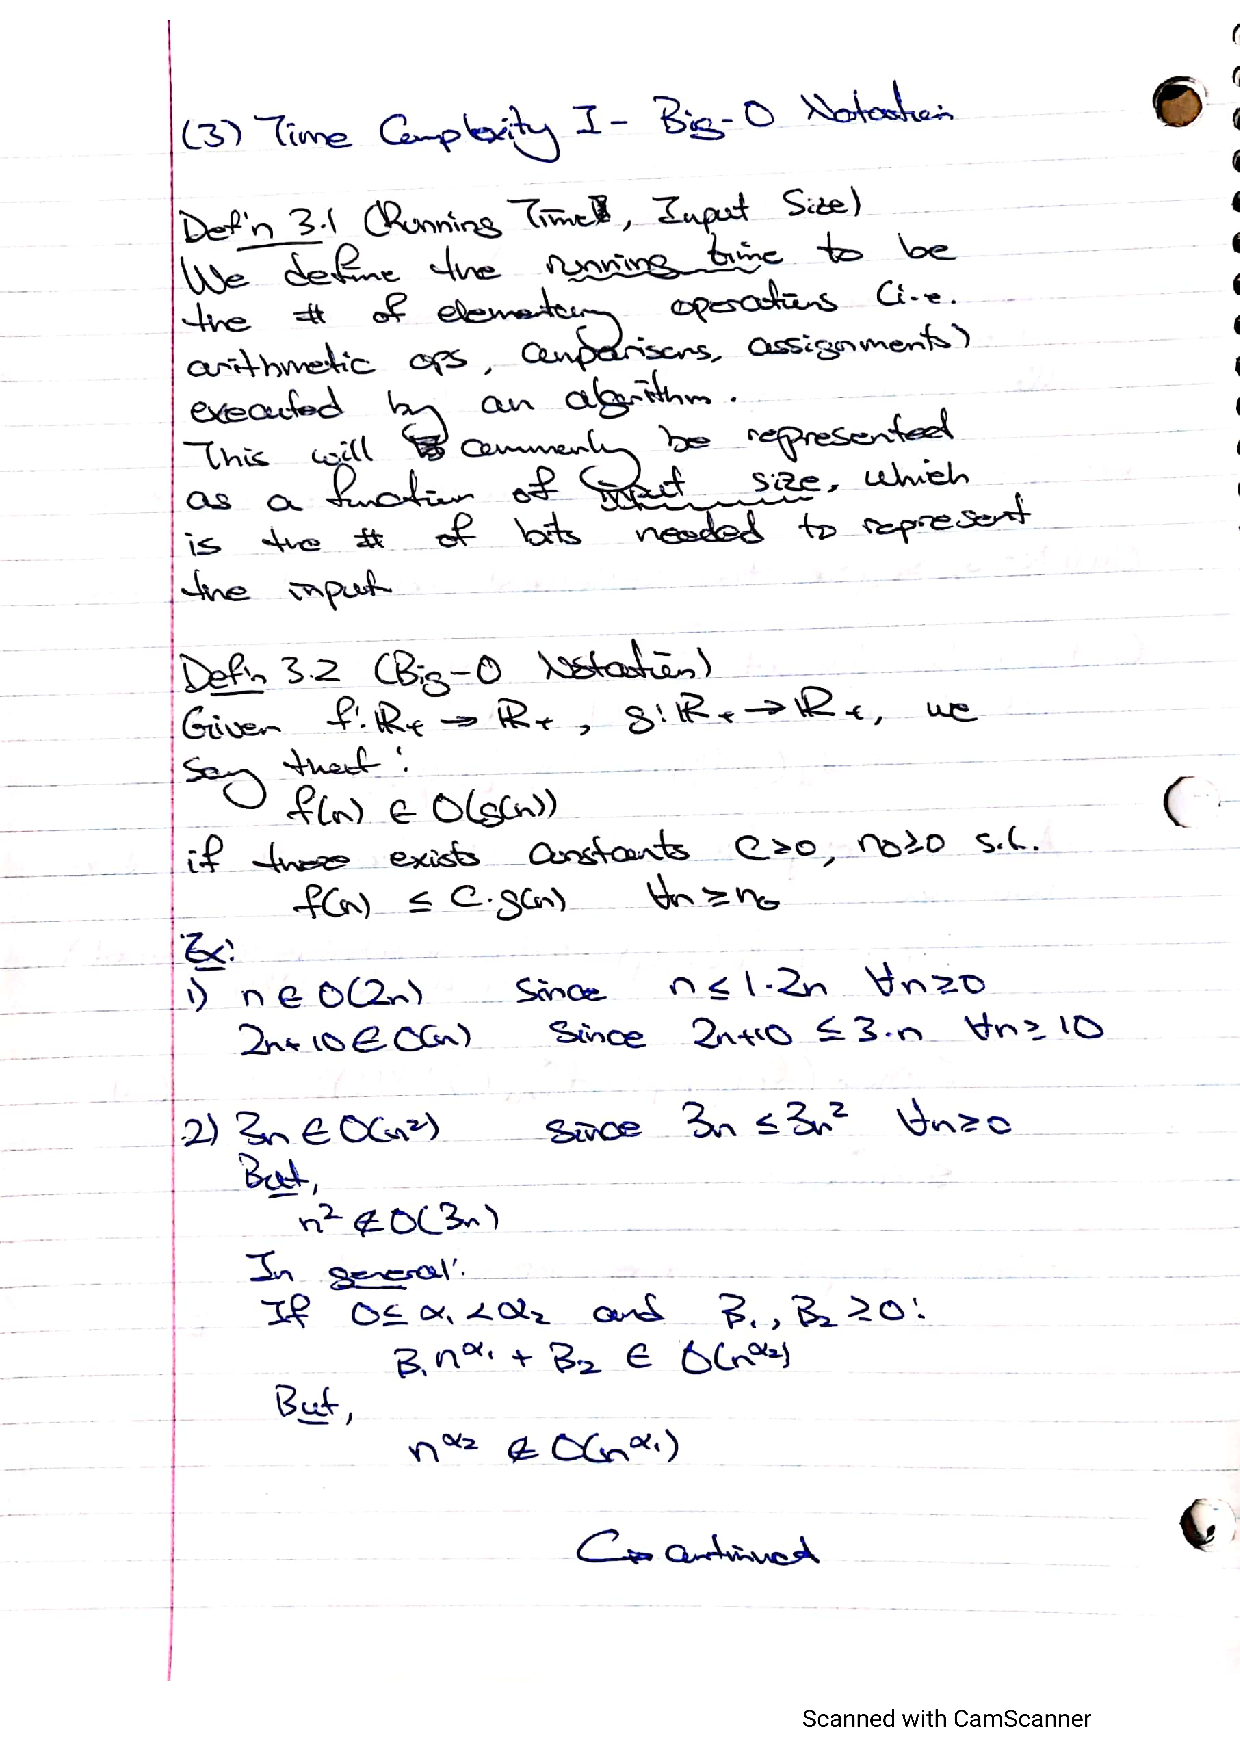
\includepdf[pages=1, pagecommand={\thispagestyle{plain}\section{Planarity}}]{sections/sec3.pdf}
\includepdf[pages=2-, pagecommand=\thispagestyle{plain}]{sections/sec3.pdf}
\clearpage

\includepdf[pages=1, pagecommand={\thispagestyle{plain}\section{Matchings}}]{sections/sec4.pdf}
\includepdf[pages=2-, pagecommand=\thispagestyle{plain}]{sections/sec4.pdf}
\clearpage

\end{document}
